\chapter{The Graphic User Interface} % (fold)
\label{cha:the_graphic_user_interface}

\section{Home Tab} % (fold)
\label{sec:tabs}
	As shown in Figure~\ref{fig:hometab}, home tab is created for adding new event to the app. The default view for user entering the app is Figure~\ref{fig:guideview}. \\
	
	Figure~\ref{fig:guideview} gives a short tutorial for user. If the user chooses the plus sign in navigation bar, a another blank view should show up. After tapping on the camera icon, Figure~\ref{fig:pickaction} will display an action list including ``Use Last Photo Taken'', ``Take Photo'', ``Choose from Library'' and ``Cancel''. For instance, we choose ``Take Photo'', the app should pop up a modal and let user take picture of food. A modal like Figure~\ref{fig:moveandscale} should appear for user to move and scale the photo to a right position and size. Figure~\ref{fig:didpick} will show up after scaling step. If no photo is chosen, a warning will show up to alert user add a photo first. Tap on next to move to next view Figure~\ref{fig:moreinfo}. In this view, a form is created for user to fill in location information, date, tags, comment and rate. Since the user just starts to eat, comment and 
rate field can be empty for now. Other fields should be filled correctly in this view because the user won't be able to edit all the other fields. In Figure~\ref{fig:locationpicker}, the location list is generated through Foursquare API. Foursquare API is chosen here because it has a good reputation in both academic and industry world. By passing current longitude and latitude, we're able to have a venue list based the distance.

\begin{figure}
    \centering
    \SetFigLayout{3}{3}
    \subfigure[Guide View]{
	\label{fig:guideview}
	
\includegraphics[width=\figwidth, totalheight=\figheight, keepaspectratio]{./screenshots/home.png}} \hfill
    \subfigure[Pick Action]{
	\label{fig:pickaction}
	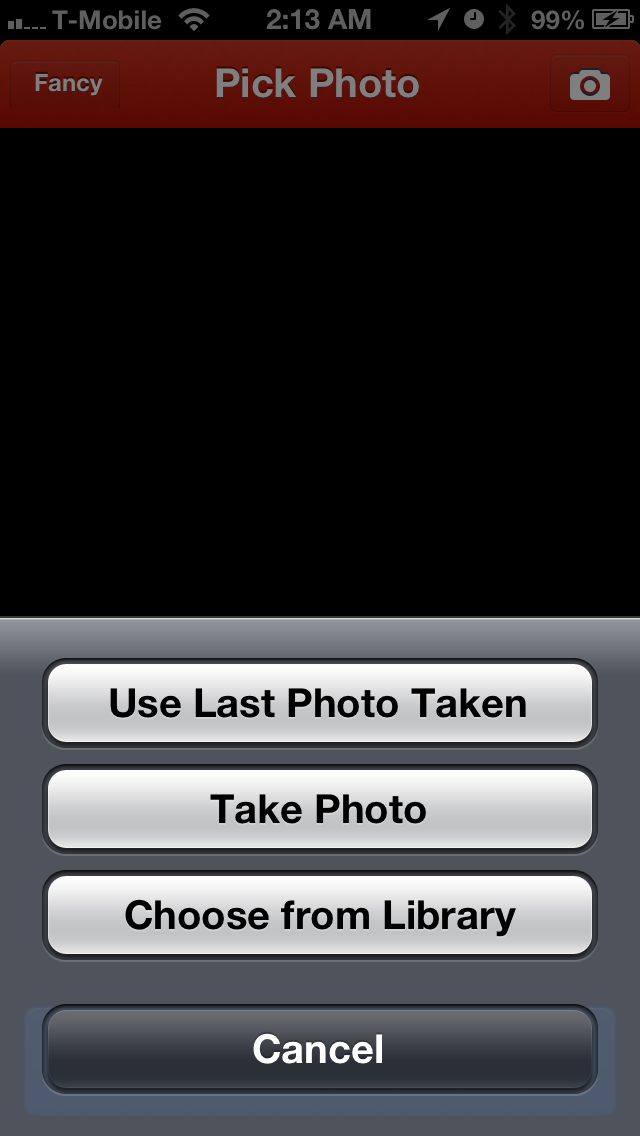
\includegraphics[width=\figwidth, totalheight=\figheight, keepaspectratio]{./screenshots/home-pickaction.png}} \hfill
	\subfigure[Move and Scale]{
	\label{fig:moveandscale}
	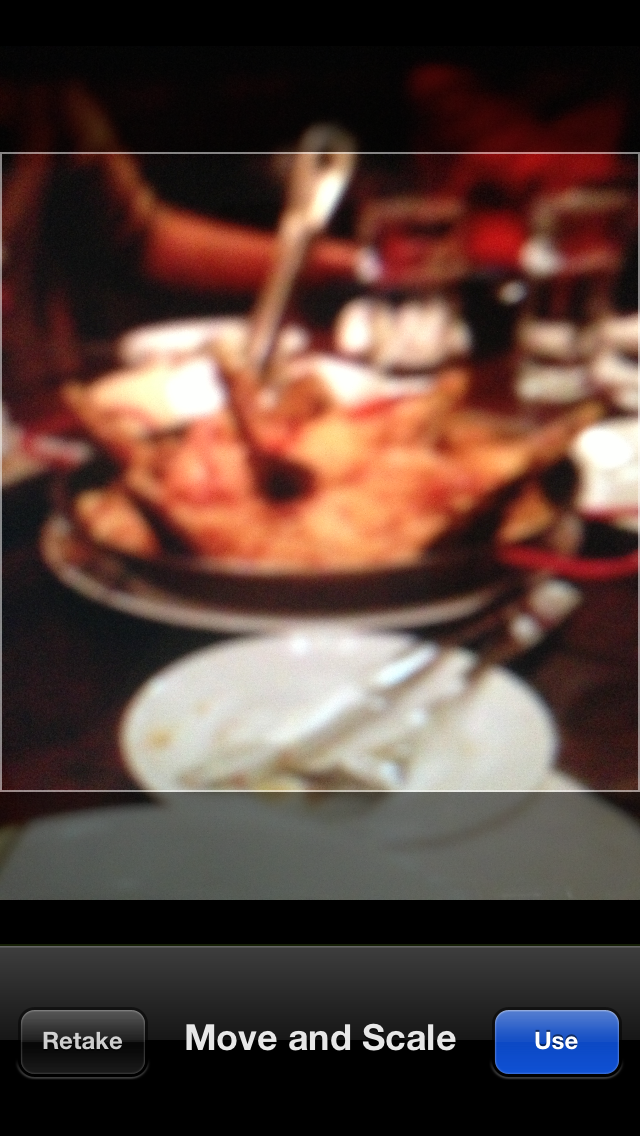
\includegraphics[width=\figwidth, totalheight=\figheight, keepaspectratio]{./screenshots/home-moveandscale.png}} \hfill \\
    \subfigure[After Picking]{
	\label{fig:didpick}
	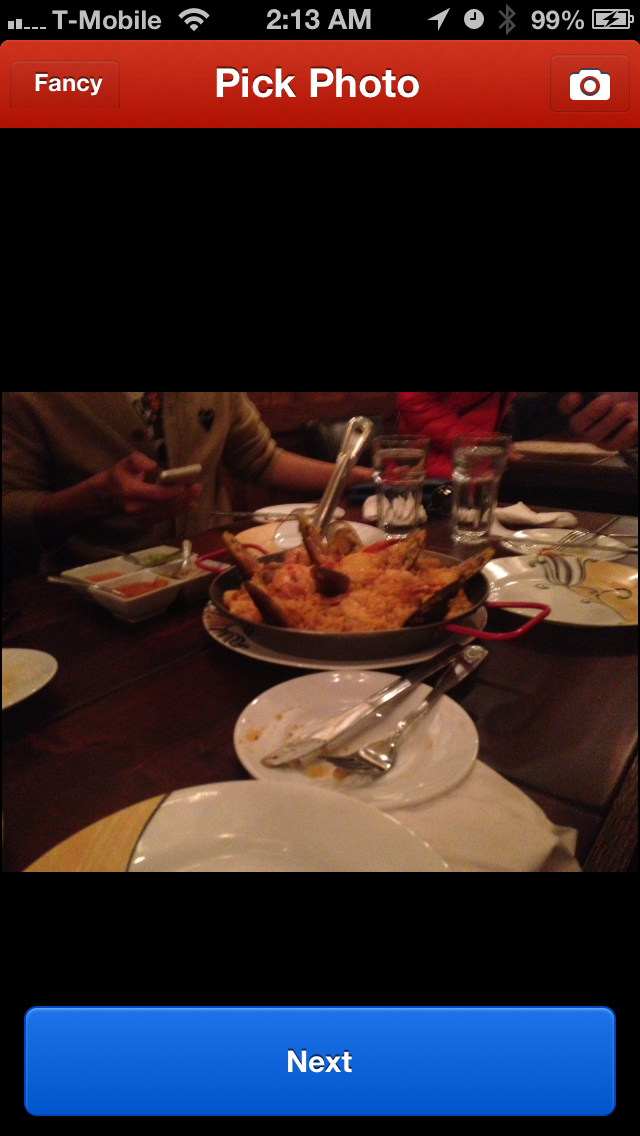
\includegraphics[width=\figwidth, totalheight=\figheight, keepaspectratio]{./screenshots/home-didpick.png}} \hfill
	\subfigure[Event Form]{
	\label{fig:moreinfo}
	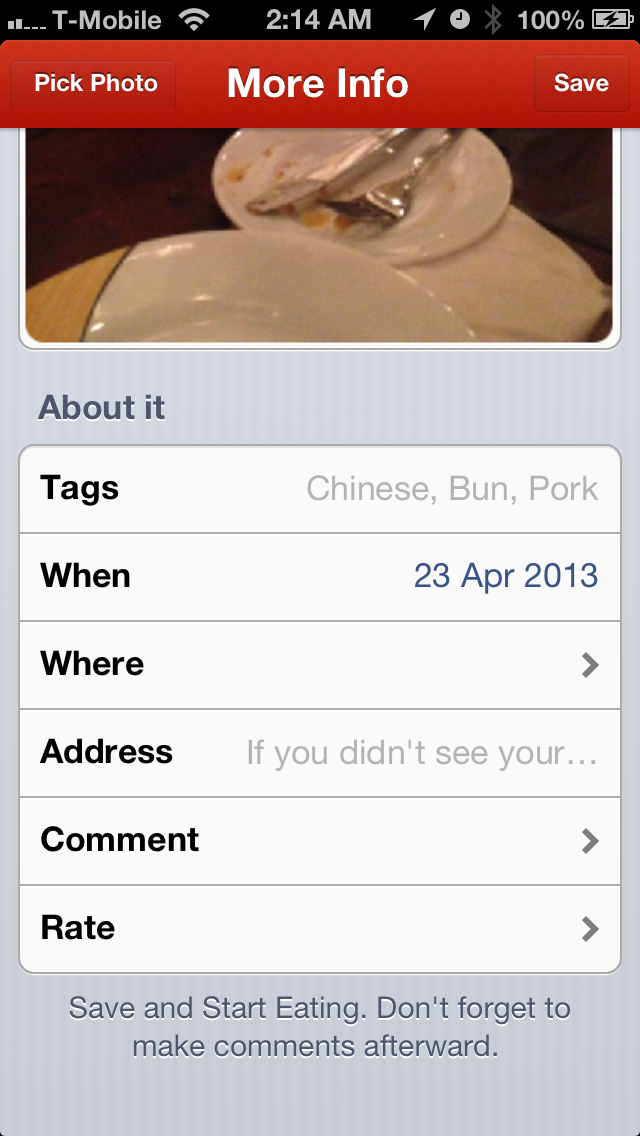
\includegraphics[width=\figwidth, totalheight=\figheight, keepaspectratio]{./screenshots/home-moreinfocontd.png}}   \hfill
    \subfigure[Date Picker]{
	\label{fig:datepicker}
	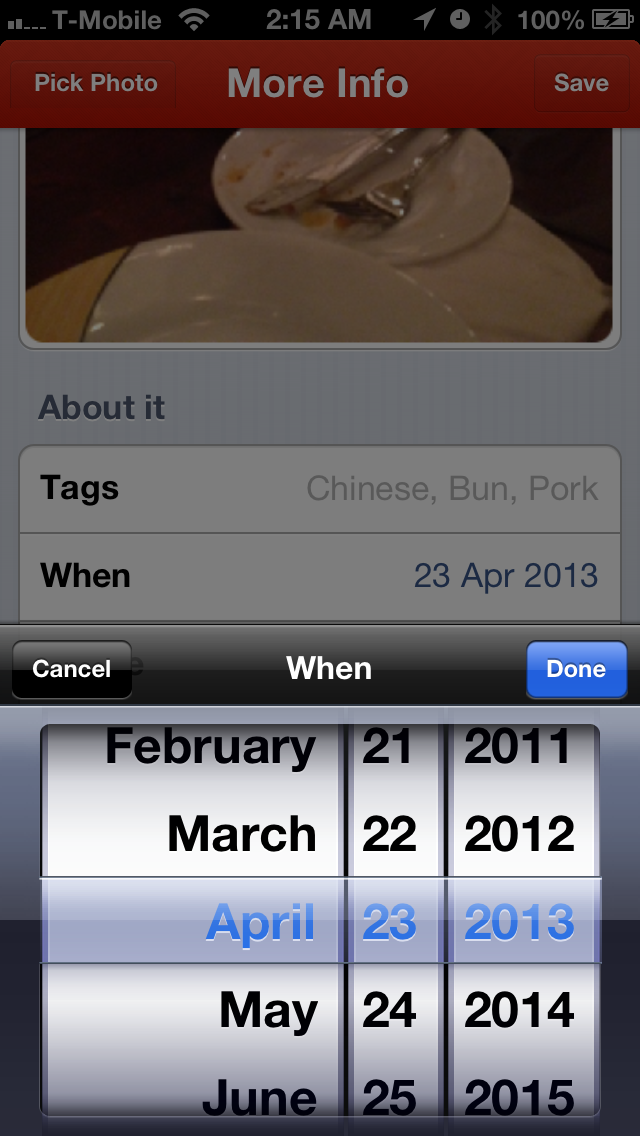
\includegraphics[width=\figwidth, totalheight=\figheight, keepaspectratio]{./screenshots/home-when.png}} \hfill \\
    \subfigure[Location Picker]{
	\label{fig:locationpicker}
	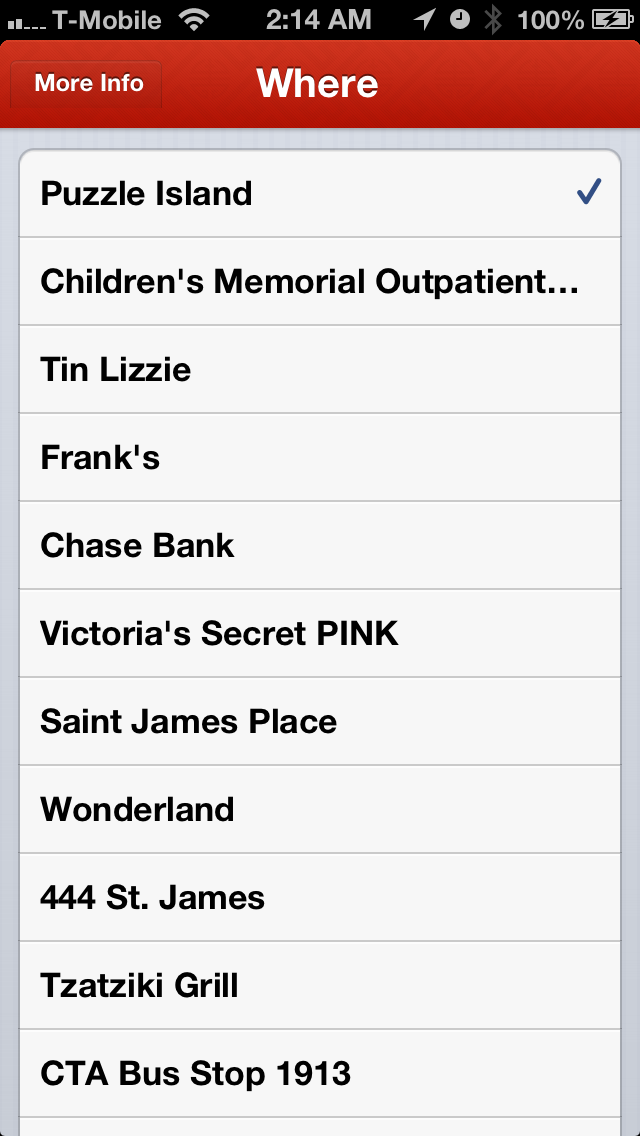
\includegraphics[width=\figwidth, totalheight=\figheight, keepaspectratio]{./screenshots/home-where.png}} \hfill
	\subfigure[Comment Editor]{
	\label{fig:commenteditor}
	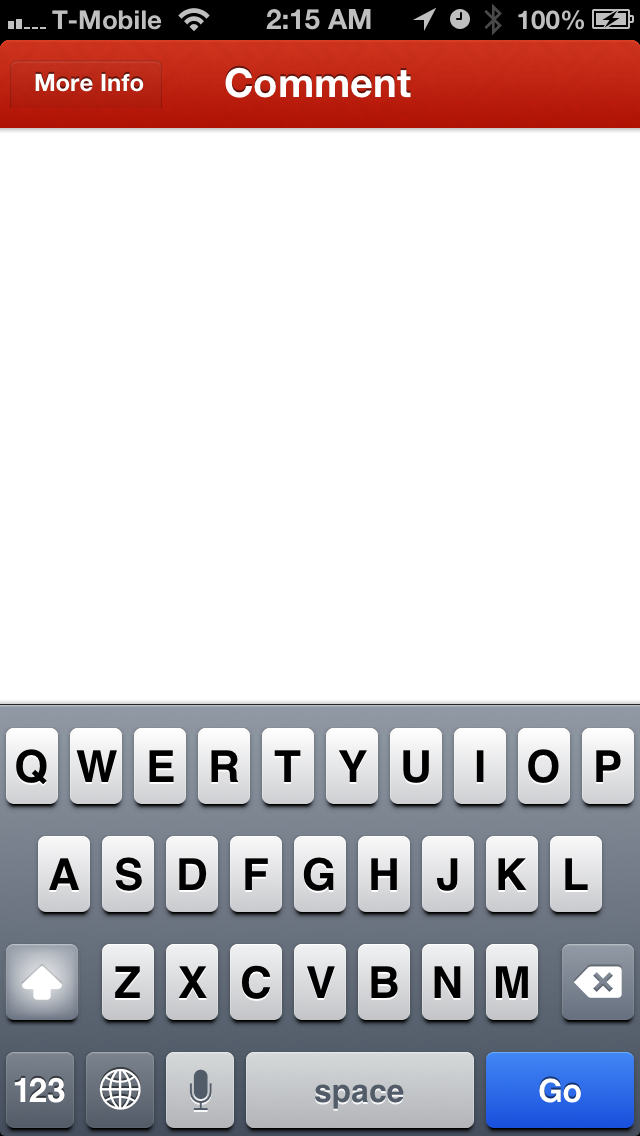
\includegraphics[width=\figwidth, totalheight=\figheight, keepaspectratio]{./screenshots/home-comment.png}}  \hfill
	\subfigure[Rate Picker]{
	\label{fig:ratepicker}
	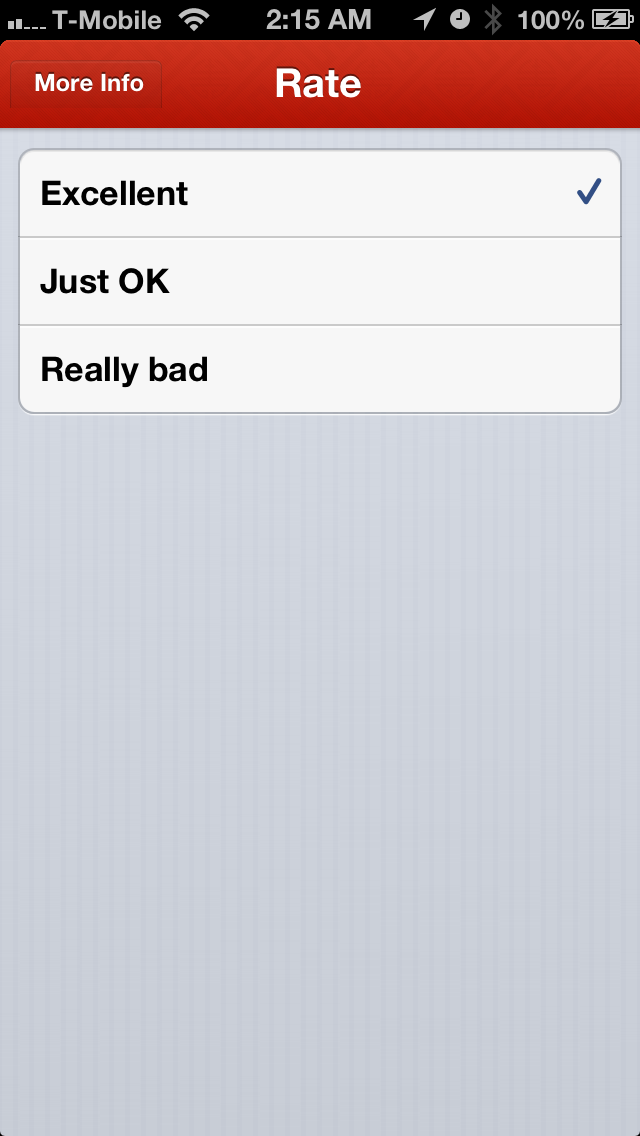
\includegraphics[width=\figwidth, totalheight=\figheight, keepaspectratio]{./screenshots/home-rate.png}} \hfill
	\caption{Home Tab View}
	\label{fig:hometab}
\end{figure}



% section tabs (end)

\section{Food List Tab} % (fold)
\label{sec:foodie_list_tab}

   In food list tab, it fetches a list of food events ordered by creation date. Figure~\ref{fig:foodlist} shows some events. On each table cell, it shows a thumbnail, time string and string of the event. And a green menu pop up button is created for sharing with social media(Figure~\ref{fig:foodlist-share}) and updating comment(Figure~\ref{fig:foodlist-comment}) or rate(Figure~\ref{fig:foodlist-rate}). \\
   
   After choosing one event, a detail view of the event will appear as shown in Figure~\ref{fig:foodlist-detail} and Figure~\ref{fig:foodlist-detailcontd}. You could see all the detailed information when you create the event. In the top navigation bar, a share button is displayed for user to share the event with friends. If the user chooses twitter, it'll check if he is logged in or not. After making sure the user have a twitter account, Figure~\ref{fig:foodlist-twitter} will appear. The comment and photo is generated by the app. Simply tap on send, and the event will be shared. \\
   

\begin{figure}
    \centering
    \SetFigLayout{3}{3}
    \subfigure[Food List]{
	\label{fig:foodlist}
	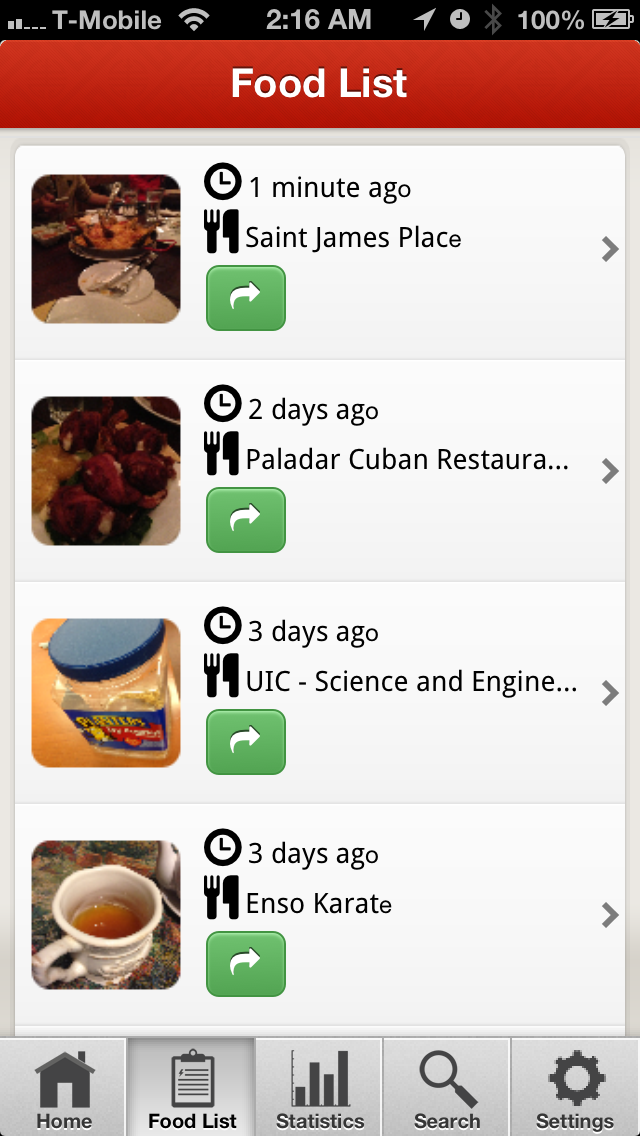
\includegraphics[width=\figwidth, totalheight=\figheight, keepaspectratio]{./screenshots/foodlist.png}} \hfill
	\subfigure[Menu Popup]{
	\label{fig:foodlist-menu}
	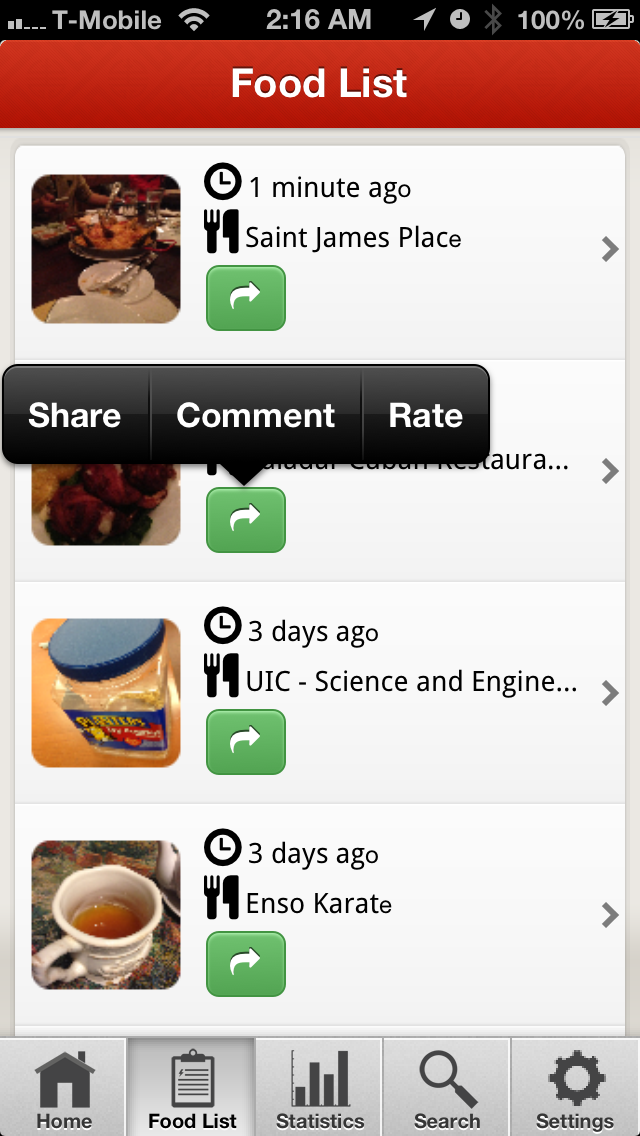
\includegraphics[width=\figwidth, totalheight=\figheight, keepaspectratio]{./screenshots/foodlist-menupop.png}} \hfill 
	\subfigure[Comment Editor]{
	\label{fig:foodlist-comment}
	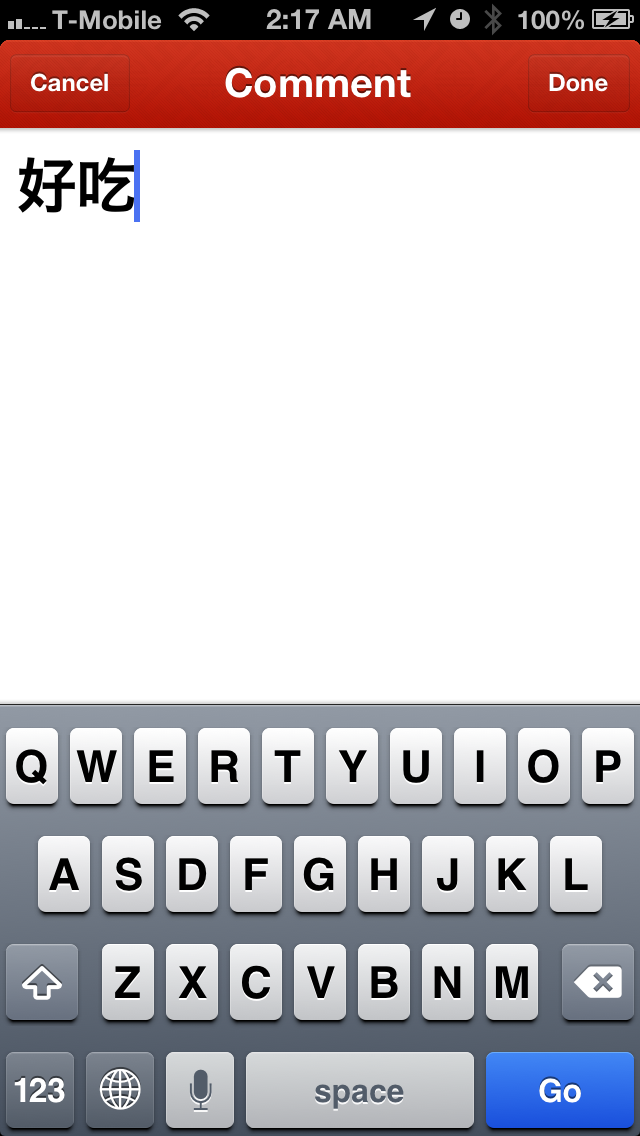
\includegraphics[width=\figwidth, totalheight=\figheight, keepaspectratio]{./screenshots/foodlist-comment.png}} \hfill \\
    \subfigure[Rate Action Sheet]{
	\label{fig:foodlist-rate}
	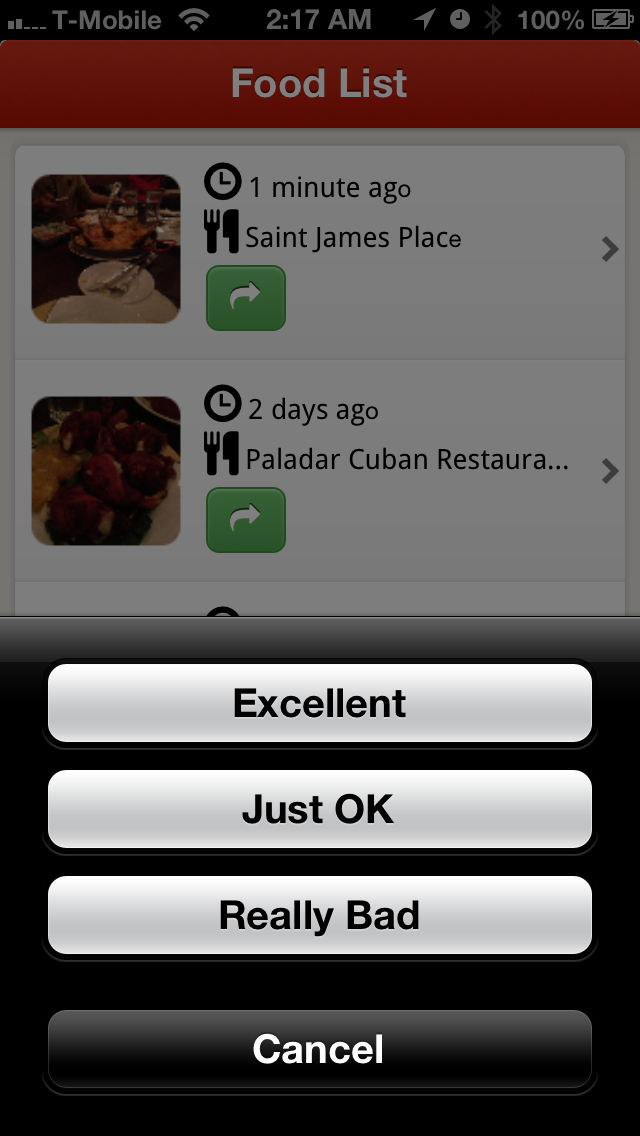
\includegraphics[width=\figwidth, totalheight=\figheight, keepaspectratio]{./screenshots/foodlist-rate.png}} \hfill
	\subfigure[Sharing Activity Controller]{
	\label{fig:foodlist-share}
	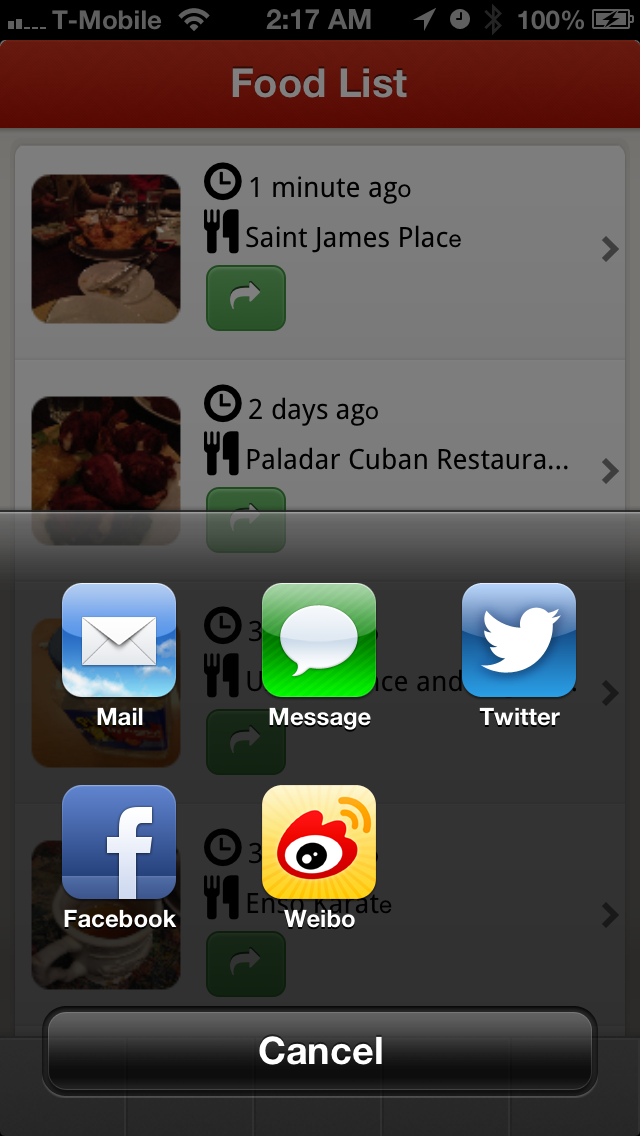
\includegraphics[width=\figwidth, totalheight=\figheight, keepaspectratio]{./screenshots/foodlist-share.png}} \hfill 
	\subfigure[Detail View]{
	\label{fig:foodlist-detail}
	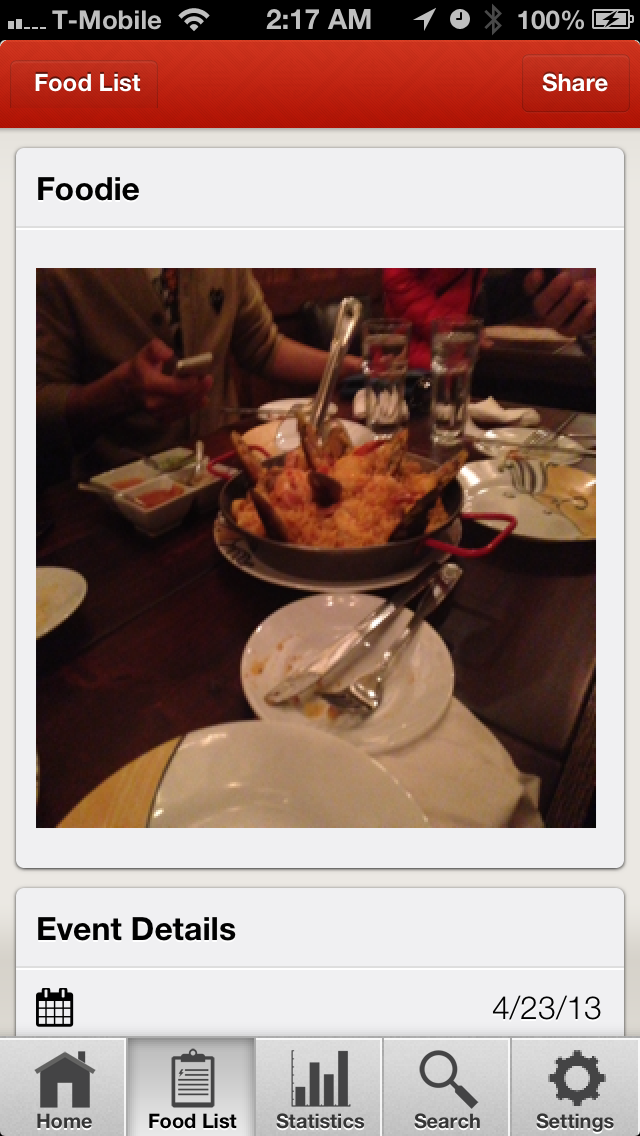
\includegraphics[width=\figwidth, totalheight=\figheight, keepaspectratio]{./screenshots/foodlist-detail.png}} \hfill \\
	\subfigure[Detail View Cont'd]{
	\label{fig:foodlist-detailcontd}
	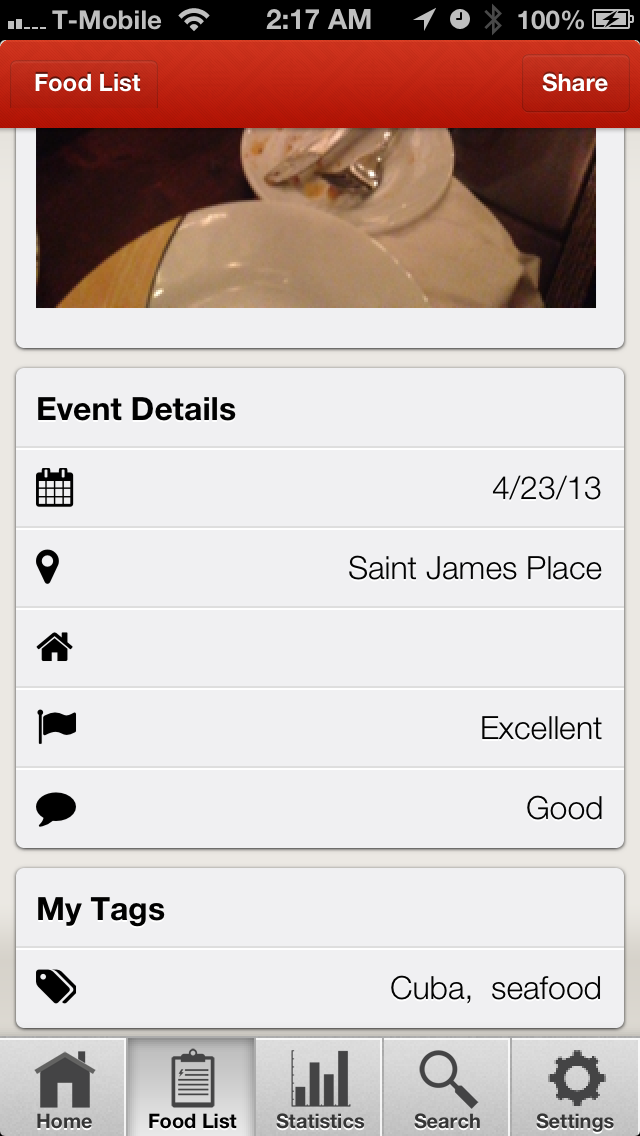
\includegraphics[width=\figwidth, totalheight=\figheight, keepaspectratio]{./screenshots/foodlist-detailcontd.png}} \hfill
	\subfigure[Twitter]{
	\label{fig:foodlist-twitter}
	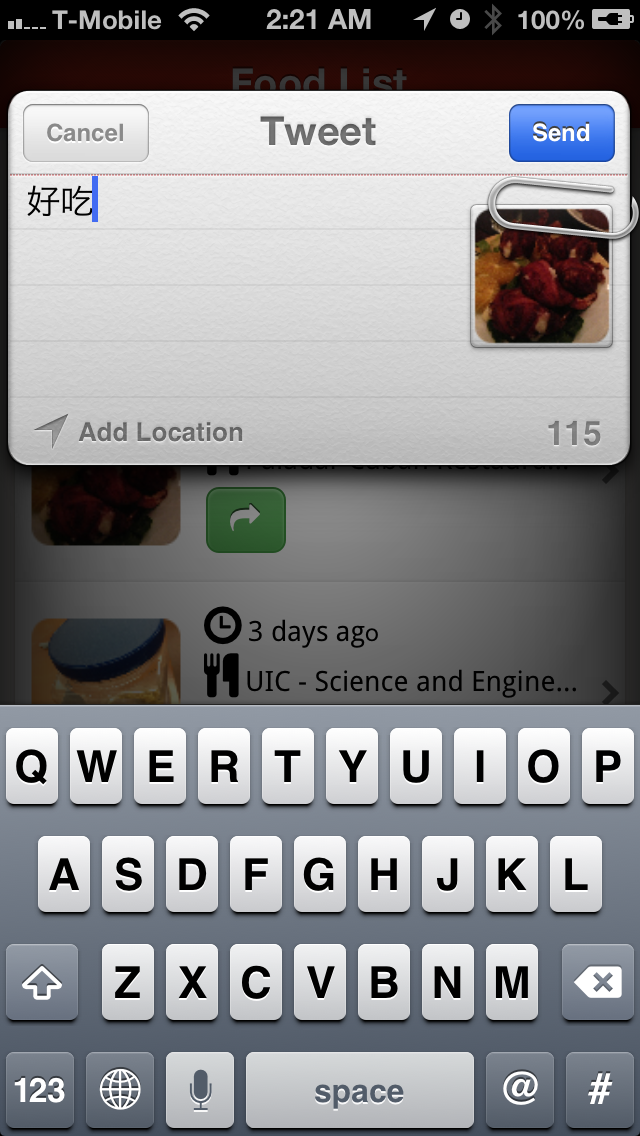
\includegraphics[width=\figwidth, totalheight=\figheight, keepaspectratio]{./screenshots/foodlist-twitter.png}} \hfill
	\subfigure[Delete View]{
	\label{fig:foodlist-delete}
	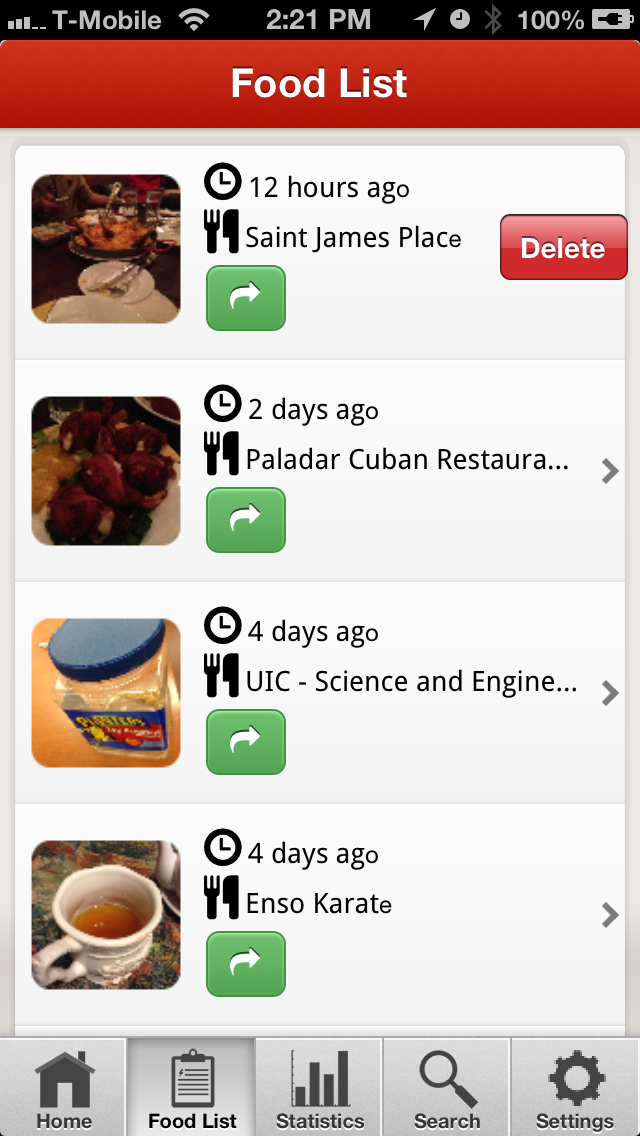
\includegraphics[width=\figwidth, totalheight=\figheight, keepaspectratio]{./screenshots/foodlist-delete.png}} \hfill
	\caption{Foodie List Tab View}
	\label{fig:foodielisttab}
\end{figure}

% subsection foodie_list_tab (end)

\section{Stats Tab} % (fold)
\label{sec:stats_tab}

Statistics tab is supposed to give the user an overview of all events he created. As shown in Figure~\ref{fig:stats}, ``Rates'' are clustered in different categories. All the tags are counted and shown in the table. The total number of places are shown in the table as well. In this way, the user can easily get an idea of what kind of places and food he likes.
  
\begin{figure}
	\centering
    \SetFigLayout{1}{1}
    {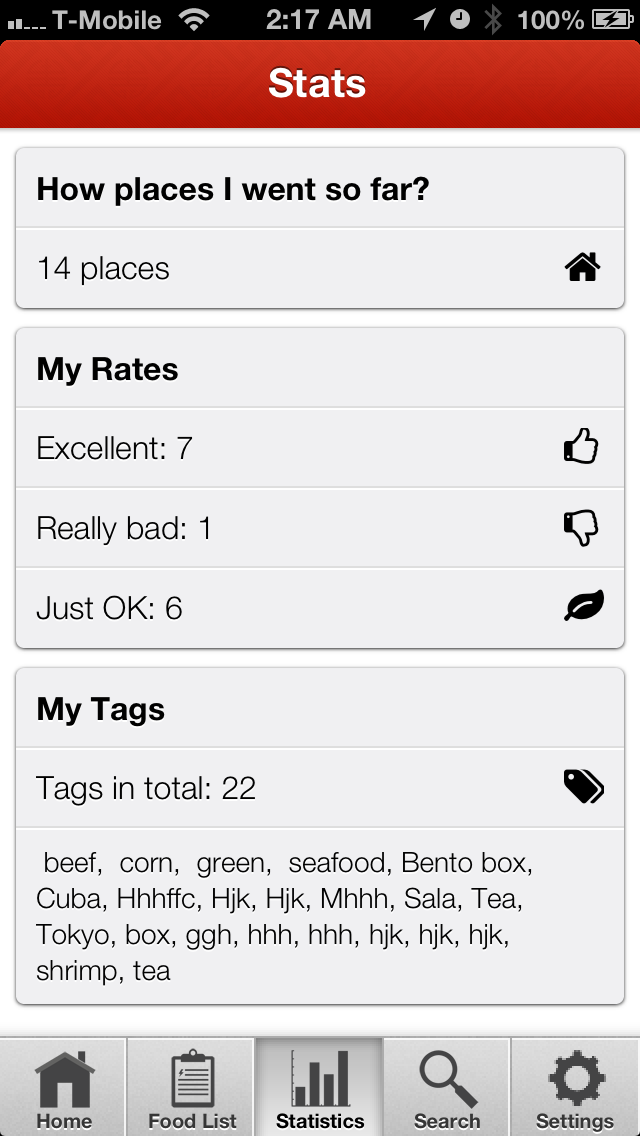
\includegraphics[%
    width=\figwidth, totalheight=\figheight, keepaspectratio]{./screenshots/stats.png}}
    \caption{Statistics Tab View}
	\label{fig:stats}
\end{figure}

% subsection stats_tab (end)
\section{Map Tab} % (fold)
\label{sec:map_tab}

In Figure~\ref{fig:map}, all the event locations are labeled with red pins. By default, it is showing the events around your current location. But you could also change your view by passing address in Figure~\ref{fig:map-address}. After choosing a location in the list, the tableview will be dismissed and the new central region will be the location you chose. 

\begin{figure}
	\centering
    \SetFigLayout{1}{2}
	\subfigure[Map]{
	\label{fig:map}
	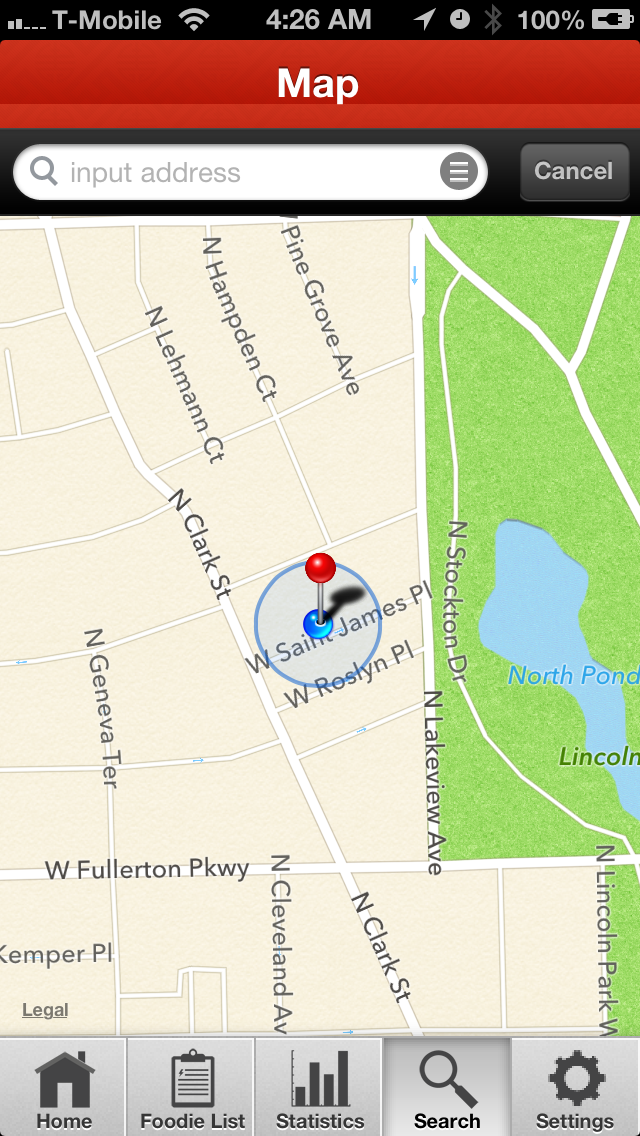
\includegraphics[width=\figwidth, totalheight=\figheight, keepaspectratio]{./screenshots/map.png}} \hfill
	\subfigure[Address Searching]{
	\label{fig:map-address}
	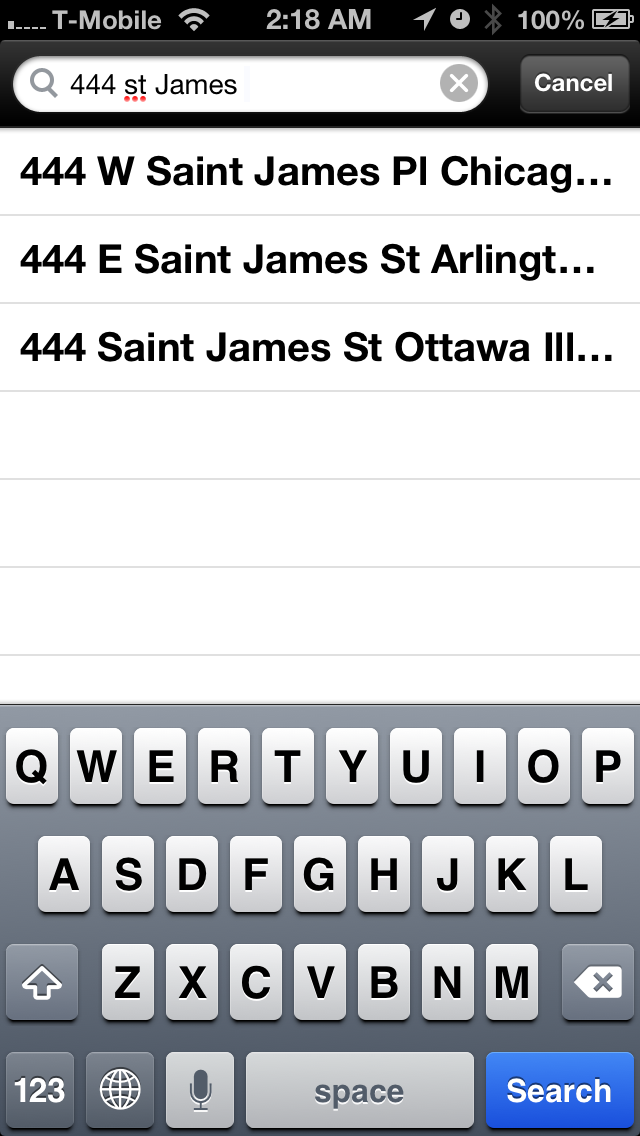
\includegraphics[width=\figwidth, totalheight=\figheight, keepaspectratio]{./screenshots/map-address.png}} \hfill
    \caption{Map Tab View}
\end{figure}

% subsection map_tab (end)

\section{Setting Tab} % (fold)
\label{sec:setting_tab}

Setting tab provides a view to setup configurations of the app (Figure~\ref{fig:settings}). The view in this tab is a static table view built in Storyboard. A web-view controller is created to show the app website and author introduction. By turning on the save photo option, it will save the photo to a album. The feedback option is used for user to submit feedback through TestFlight. TestFlight is a online tool to do open beta testing on the fly. By hooking with TestFlight, we will be able to see all the crash reports, time durations for each session, and even ask questions to users after a checkpoint is reached.\\


\begin{figure}
	\centering
    \SetFigLayout{2}{2}
	\subfigure[Settings]{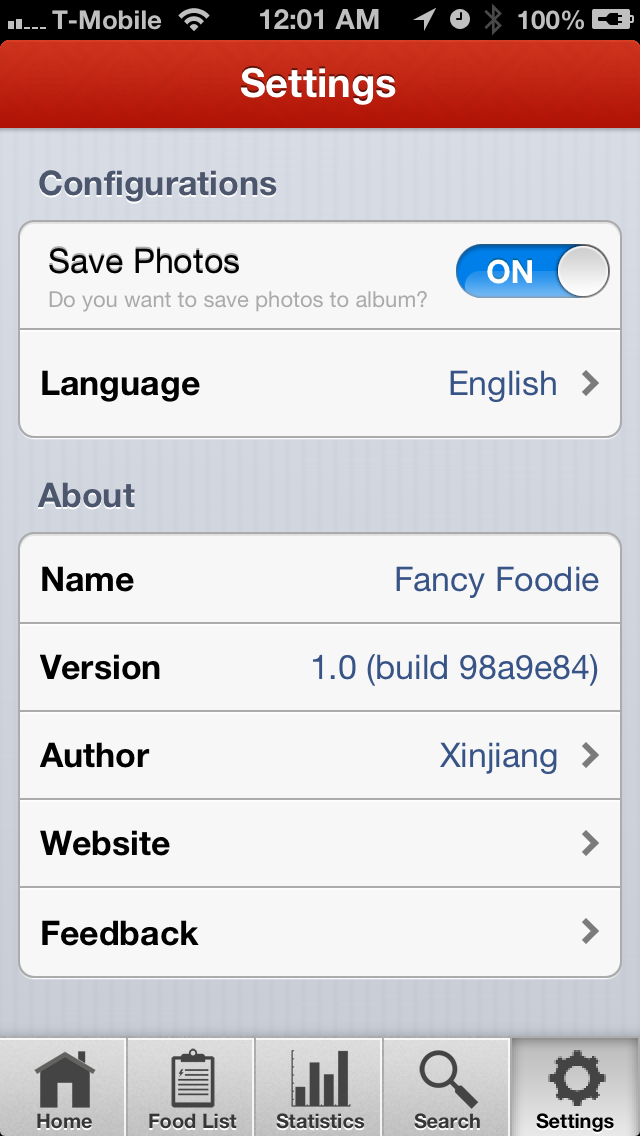
\includegraphics[width=\figwidth, totalheight=\figheight, keepaspectratio]{./screenshots/settings.png}} \hfill
	\subfigure[Save to Album]{
	\label{fig:album}
	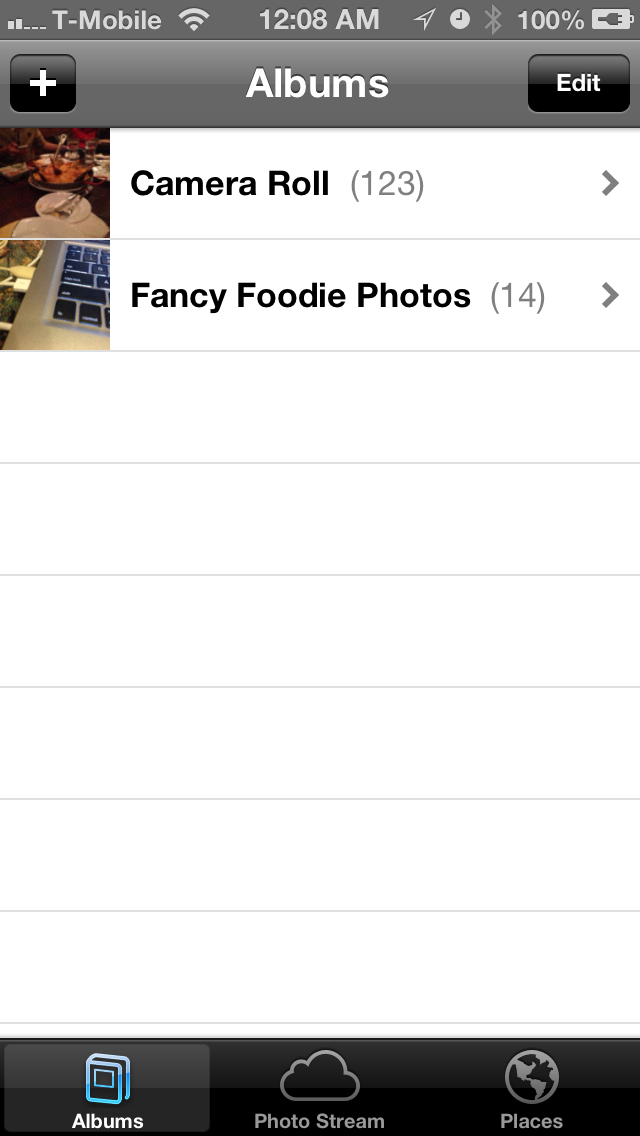
\includegraphics[width=\figwidth, totalheight=\figheight, keepaspectratio]{./screenshots/settings-album.png}} \hfill \\
	\subfigure[Author Web-view]{
	\label{fig:author}
	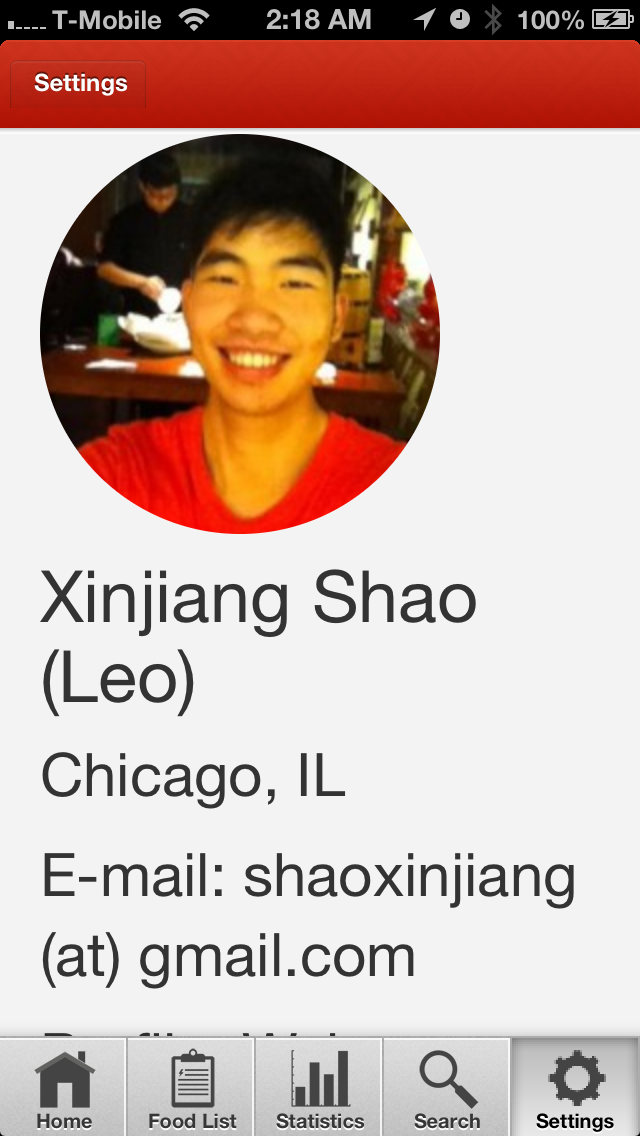
\includegraphics[width=\figwidth, totalheight=\figheight, keepaspectratio]{./screenshots/settings-author.png}} \hfill
	\subfigure[Website View]{
	\label{fig:website}
	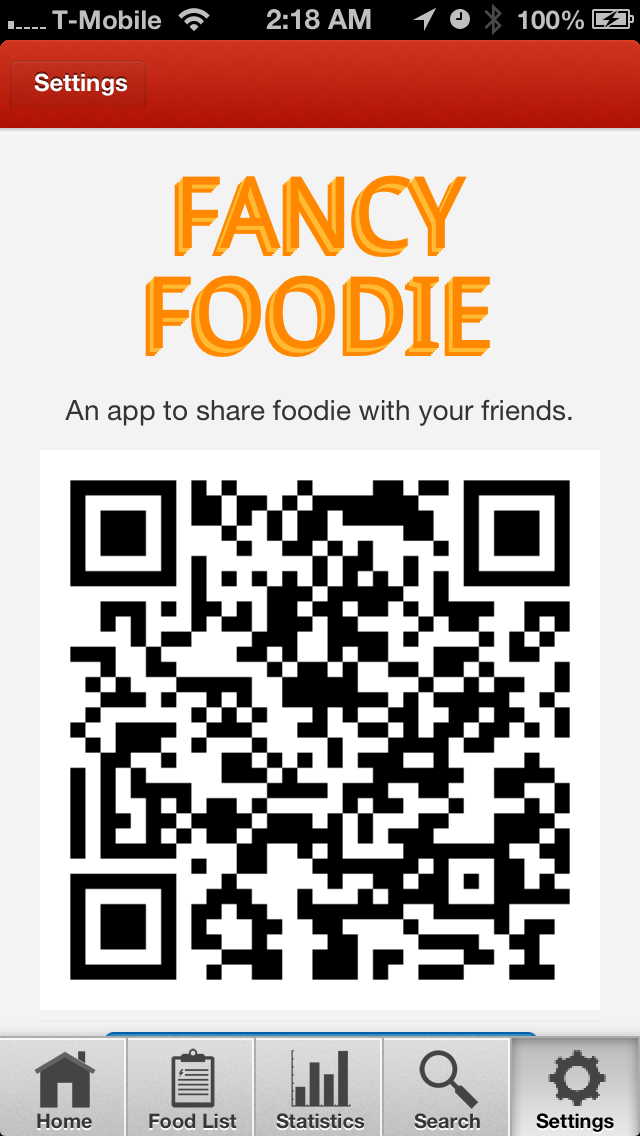
\includegraphics[width=\figwidth, totalheight=\figheight, keepaspectratio]{./screenshots/settings-website.png}} \hfill
    \caption{Setting Tab View}
	\label{fig:settings}
\end{figure}

% subsection setting_tab (end)
% chapter the_graphic_user_interface (end)